\chapter{Related Work} \label{ch:related}

\section{Related Work}

\subsection{Dataflow streaming engines}

In contrast to the standalone Timely Dataflow library, many state-of-the-art
dataflow streaming engines have been designed and engineered from the start
to run multiple current dataflow computations in a cluster. One of the
goals of this thesis was to provide such functionality for Timely Dataflow
based programs. Thus, in this section, we will mainly focus on the execution
and management aspect running multiple dataflow computations. Less focus is
put on the differences in the programming and synchronization model these 
other systems provide. Our system currently also does not provide any fault
tolerance guarantees. This is also a notable difference our system has compared
to related work, which often put heavy emphasis on providing strong fault
tolerance.

\subsubsection{Spark Streaming}

Spark Streaming \cite{sparkstreaming} is a streaming engine based on the Spark
cluster computation framework. Spark Streaming executes streaming dataflow
computations by turning them into stateless, fault-tolerant batch computations.
These batches are submitted as tasks to the underlying Spark engine. \cite{spark} 

\paragraph{Process Model}

In Spark, computational tasks work is modeled as transformations on partitioned
collections of records called \emph{resilient distribute datasets}. The
runtime schedules the execution of the transformations on a distributed set of
worker nodes. By tracking the lineage of transformations, Spark is able to
recover computations by reissuing lost transformations. Based on the model,
Spark Streaming models stateful, conceptually continuous dataflow computations
as small stateless microbatches.

This model of execution is very different from Timely's continuous operator
model. In Timely, both the operator scheduling and the data of the
computation are managed directly by the workers themselves, which are hosted
by long living operating system processes. In Spark however, the data and code
is managed by the system. Because of this, Spark is not only able provide strong
fault tolerance by reissuing failed computations, Spark is also able to load
balance concurrently running streams and mitigate stranglers. While we currently
do not offer these features, Timely does achieve much lower latencies than
Spark Streaming, which is mostly enabled by the fact that every Timely
worker manages itself independently.

%TODO driver processs

\subsubsection{Storm \& Heron}

Heron \cite{heron} is the API-compatible successor of the Storm \cite{storm}
streaming dataflow engine.
Both Storm and Heron call their dataflow computations \emph{topologies}, which 
are directed acyclic graphs of spouts (stream sources) and bolts
(stream transformers). Parallelism is achieved by the user specifying the
number of instances for each bolt and spout, as well as the partitioning
strategy between them.

\paragraph{Process Model}

The process model of Storm is very similar to our approach: A topology
(roughly corresponding to a query in our system) is executed by multiple
\emph{worker processes}. These are operating system processes which distributed
over different machines, thus similar to our query proceses. Every machine hosts
a \emph{supervisor}, which not only monitors the local worker processes, but also spawns new worker
processes on behalf of the \emph{Nimbus}, making Storm's supervisors similar to our executors.
The Nimbus is a central process to which new topologies are submitted, mirroring our coordinator.

Heron mostly differs from Storm in its internal architecture. Most notably, in
Heron every spout or bolt now runs in its own operating system process. All processes
belonging to the same topology are grouped together in operating system containers.
The motivation for this change are reported to be better debug-ability
and simpler resource management. The authors also state that their topologies
seldom have more than three stages (i.e. bolts/spouts). We believe that such
an architecture would not make much sense for Timely, as its operators are typically
more numerous and more lightweight.

Another major change from Storm's architecture
is the fact Heron does not have a central coordinating process anymore. Being
a single point of failure and a bottleneck, the Nimbus was considered to be a
flawed design. Heron thus replaces the old responsibilities of the Nimbus by
offloading them into a small set of independent processes. This might be something
to consider for futures extensions to our coordinator.

\subsubsection{Flink}

Flink \cite{flink} is a dataflow streaming engine for directed acyclic
dataflow graphs, however it does have support for iterative dataflows on the
outermost level. Flink interleaves control events with data records, which
are used for progress tracking and fault tolerance, which is done through
snapshots. Progress tracking is implemented with global \emph{low watermarks}, which
denote the minimum timestamp which can be emitted at the sources of the
topology, enabling Flink to perform out-of-order processing.

\paragraph{Process Model}

The runtime architecture of Flink also uses a central process called the
\emph{Job Manager}, which accepts and manages computations submitted by
the client. The Job Manager takes the user submitted code, translates it into
an execution plan and potentially optimizes it.

The computations themselves are executed inside worker processes called
\emph{Task Managers}. Task managers provide a similar function like our executors, in that
they are processes distributed over potentially multiple machines and provide access to
computational resources. They can be dynamically added and announce them selves at the
job manager. However, in contrast to our executors, task managers directly execute the
operators and implements the exchange data between them. In our system, this task is done by the
query library and the Timely runtime. For resource management purposes, each task manager provides
a predefined number of task slots. These typically correspond with the number of CPU cores,
though a single slot might host multiple threads. The available memory is also distributed
equally between the task slots of an task manager. The submitted dataflow computation is split up
in multiple subtasks (typically corresponding to an operator), and each subtask is assigned
to a task slot. Subtasksfrom the same job (i.e. submission) can share a task slot
if the operator supports it, which is useful for example for pipelined operators which don't
require any exchange of data with operators running in other task slots.
Because task managers can have multiple task slots, they can run operators from different
computations within the same operating system process, similar to Spark Streaming. Unlike
Spark Streaming, but like Heron and our system, these operators are however long-lived
and do not migrate to other task slots, as Flink also implements a continuous operator model.

\subsection{Dataflow composition}

\subsubsection{Kafka}

Kafka \cite{kafka} is a distributed platform for accumulating and sharing streams. It provides
a publish/subscribe service for potentially partitioned topics. Producers append
their data to one or more partition, allowing subscribers to read from it.
The data within a partition is stored persistently, allowing subscribers to
read all previously published data sequentially and continue where they left
of in case of failure. The data within a partition is ordered, however there
is no defined ordering across multiple partitions of the same topic. Recent
versions of Kafka also supports the assignment of event timestamps to messages.

\paragraph{Integration with Dataflow Engines}

Both Spark Streaming and Flink provide official connectors for Kafka, allowing
dataflow computations to stream data from or to Kafka topics. Flink supports
the extraction of timestamps from topics, allowing a partition
to contain out-of-order data. Similar to our system, Flink also provides a
mechanism to exact watermarks from Kafka sources, which like our system
is able to unify the progress tracking information from multiple sources.

In some ways, Kafka is very similar to our publish/subscribe as we also expose
potentially partitioned streams from which consumers, such as dataflow programs,
can subscribe to. In contrast to Kafka, we have a strict one-to-one mapping between stream
partitions and topics. Stream partitions in our system are only grouped together
by following naming conventions on the topic name. 
 
Another difference between Kafka and our system is that Kafka's subscribers are
\emph{pulling} data from their source, whereas in our system data is \emph{pushed}
from the source to the subscribers. The implication of this in our
system is that the publisher does not know anything about the progress of the
subscriber, which can lead to back-pressure issues if the subscribers are
slow.

\paragraph{Kafka Streams}
In additions to the above mentioned adapters, Kafka also provides its own
streaming engine called Kafka Streams. It provides a simple acyclic dataflow
model which uses Kafka topics and sources and sinks, thus acting as transformers.
Parallelism is achieved by instantiating the dataflow graph on multiple threads.
Partitioning of the data happens before it is fed to the individual instances
of the dataflow graph.

Like standalone Timely Dataflow, Kafka Streams is implemented as a library. It
is left to the user to deploy and launch instances of the streaming computation.

\subsubsection{MillWheel}

MillWheel \cite{millwheel} is a stream processing framework used to implement
the dataflow model proposed by Google \cite{google}. MillWheel conceptually
treats the whole system as a single dynamic dataflow graph: The nodes of the
dataflow graph are user submitted computations (i.e. operators) that are
invoked by the system on receipt of incoming data. Edges are created by the
user specifying which streams a computation consumes and produces. Streams
have uniquely assigned names.

This makes MillWheel essentially a publish/subscribe system, every individual
operator acts as a subscriber and a publisher. This is slightly different from
our system and other combinations of dataflow systems that use an external
publish/subscribe mechanism: Streams between operators are anonymous until
explicitly published, while in MillWheel all streams used to connect operators
are automatically available by for subscription by third parties.

Another difference to our approach is the fact that MillWheel lets subscriber
specify how a stream should be partitioned before it is delivered to the consumer.
Aggregation and partitioning is done according to keys, i.e. records with the
same key are always delivered to the same computation instance. Different
computations can however use different keys on the same streams, as every computation
needs to provide a key extraction function for each of its input streams.

Computations run on one or more processes distributed over a dynamic set of
machines. The assignment of computations to machines and keys to computations
is managed by the system it self. Because the system manages persistent state
on behalf of the computations, computations for a certain key can be moved
for load-balancing or restarted in the case of failures.

\begin{comment}
\begin{table}
    \myfloatalign
  \begin{tabularx}{\textwidth}{llllll} \toprule
    \tableheadline{Feature} & \tableheadline{Our System} & \tableheadline{Spark Streaming} & \tableheadline{Storm} & \tableheadline{Heron} & \tableheadline{Flink} & \tableheadline{MillWheel}\\ \midrule

    \bottomrule
  \end{tabularx}
  \caption{Summarized comparison of related work}  \label{tab:related-work}
\end{table}
\end{comment}

\cleardoublepage
\chapter{Future Work \& Conclusions} \label{ch:conclusions}

\section{Future Work}



\subsection{Extracting Query Metadata}

Our system currently treats queries for the most part as black boxes. While we
do dynamically track some information about the query such as its publications
and subscriptions, the system does not know anything about a queries internal
dataflow graph. As discussed in section \fullref{sec:runtime-graph}, Timely
itself only assembles a type-erased representation of the dataflow graph
during execution. The integrated logging framework also only exposes the
structure of the dataflow graph, but not any properties about the nodes and
edges themselves besides the name of the operators. While further instrumentation
of Timely would certainly be able to provide more insight into the dataflow
graph, solely dynamic approaches are limited in what they can do:
Rust does not provide any run-time reflection of types besides unique type
identifiers, and most operators accept user-defined functions to implement
parts of their logic. We therefore believe that some forms of static analysis
or user-provided descriptions are unavoidable for extracting precise information
about the dataflow graph. Possibles uses for more precise descriptions of the
dataflow graph of a query are described below.

\subsection{Retroactive Tapping of Dataflow Edges}

With the current publish/subscribe mechanism, query authors are required to
anticipate which operator outputs are of possible interest for subscribers. If
a certain output is not explicitly published using a publish operator, there
is no way for other queries to access it. We believe that some mechanism for
retroactively exposing dataflow edges in a running query would be useful not
only for diagnostics and manual query composition, but potentially also
for query optimization. 

We considered implementing such a feature as part
of this thesis. The design choice of topics that can be dynamically added
or removed from the catalog was also made with such a use-case in mind.
However, due to time constraints, we were not able to pursue an implementation.
In the remainder of this section, we however do present some of our
preliminary ideas.

\paragraph{Exposing Stream Handles}

We believe that it would be relatively easy to instrument Timely's in a way
that exposes it's data streams without much run-time overhead: Timely's
\lstinline{Stream<S, D>} handle internally maintains an internal
registrar which is used by successor nodes to register themselves as consumers.
When pushing data into the conceptual stream, the producer pushes the data to
all queues that have been registered on that stream. By collecting and exposing
the registrars of all edges, it would easily be possible to add new consumers
at run-time. An unresolved issue with this approach however is that this would only allow
the inspection of the \textquote{data plane} of a Timely computation. Because
progress tracking information is delivered separately, a way has to be found to
expose this information as well.

\paragraph{Processing intercepted streams}

Previous work on monitoring distributed systems such as P2 \cite{p2} and
Pivot Tracing \cite{pivot} has demonstrated powerful interfaces for
processing and querying intercepted streams of running systems.
We believe that a functionality to tap into dataflow edges of running queries would
enable similar possibilities in our system: By retroactively publishing
dataflow edges as topics, other queries could be used to monitor, diagnose or
extend a running dataflow computation.

Furthermore, the overhead of serializing intercepted tuples could be avoided
by extending the system to dynamically load code into running queries. Systems
such as Pivot Tracing and Spark are using Java's ability to dynamically load
bytecode into the running programs. For our Rust-based system we envision a
mechanism where queries are loaded as dynamic shared objects into running
computations.

\paragraph{Query optimization through derived topics}

A detailed representation of a query's dataflow graph, together with the ability
to tap into dataflow edges could also be used for query optimization. An example
of this is path deduplication: If a new incoming query perform the same
sequence of operations on the same stream of data as an already existing
query, we would like to deduplicate this work. By exploiting the fact that
topics act as semantic descriptions of streams, the system could automatically
created \emph{derived topics}. These derived topics represent the stream
generated from a sequence of operators applied to the original topic. They would
be automatically created by the system by tapping into dataflow edges of
existing queries. An example of this is shown in Figure~\ref{fig:queryoptimization}.

\begin{figure}[!htb]
  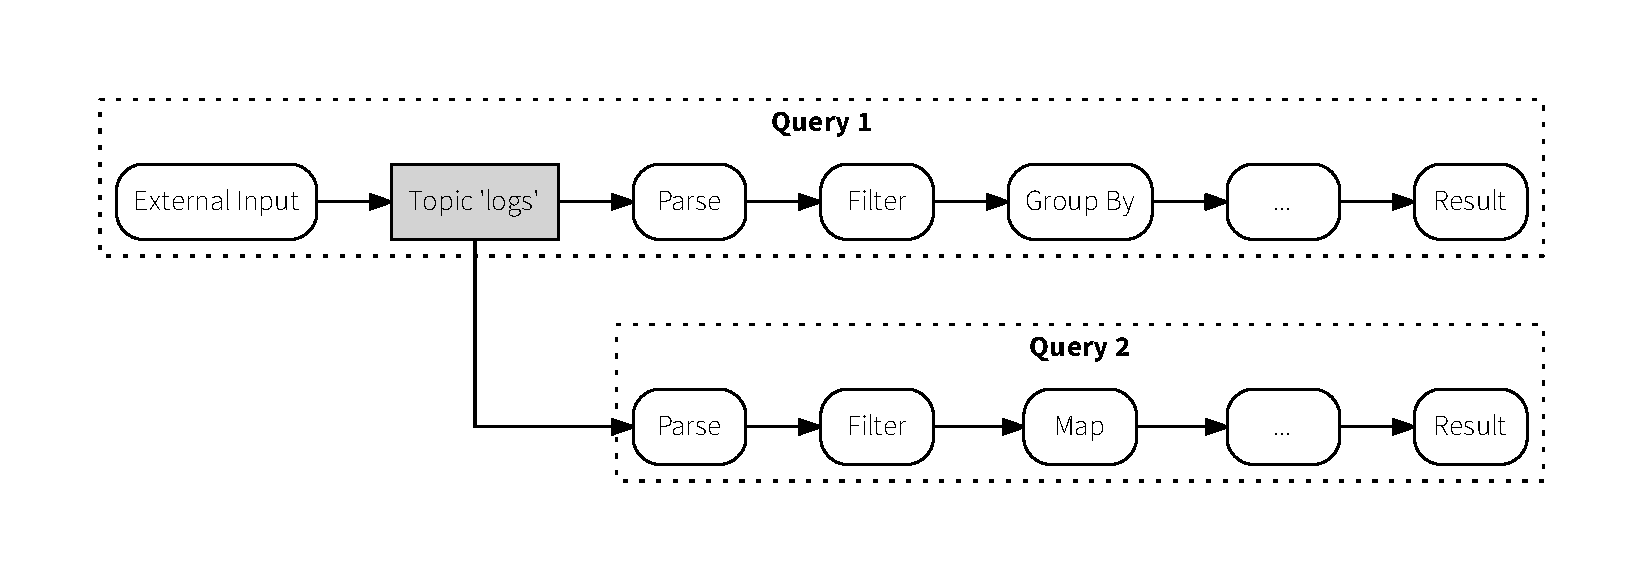
\includegraphics[scale=0.36]{figures/composition/q1q2_man}
  \vspace{-1.5em}
  \begin{center}
  $\Downarrow$
  \end{center}
  \vspace{-1.2em}
  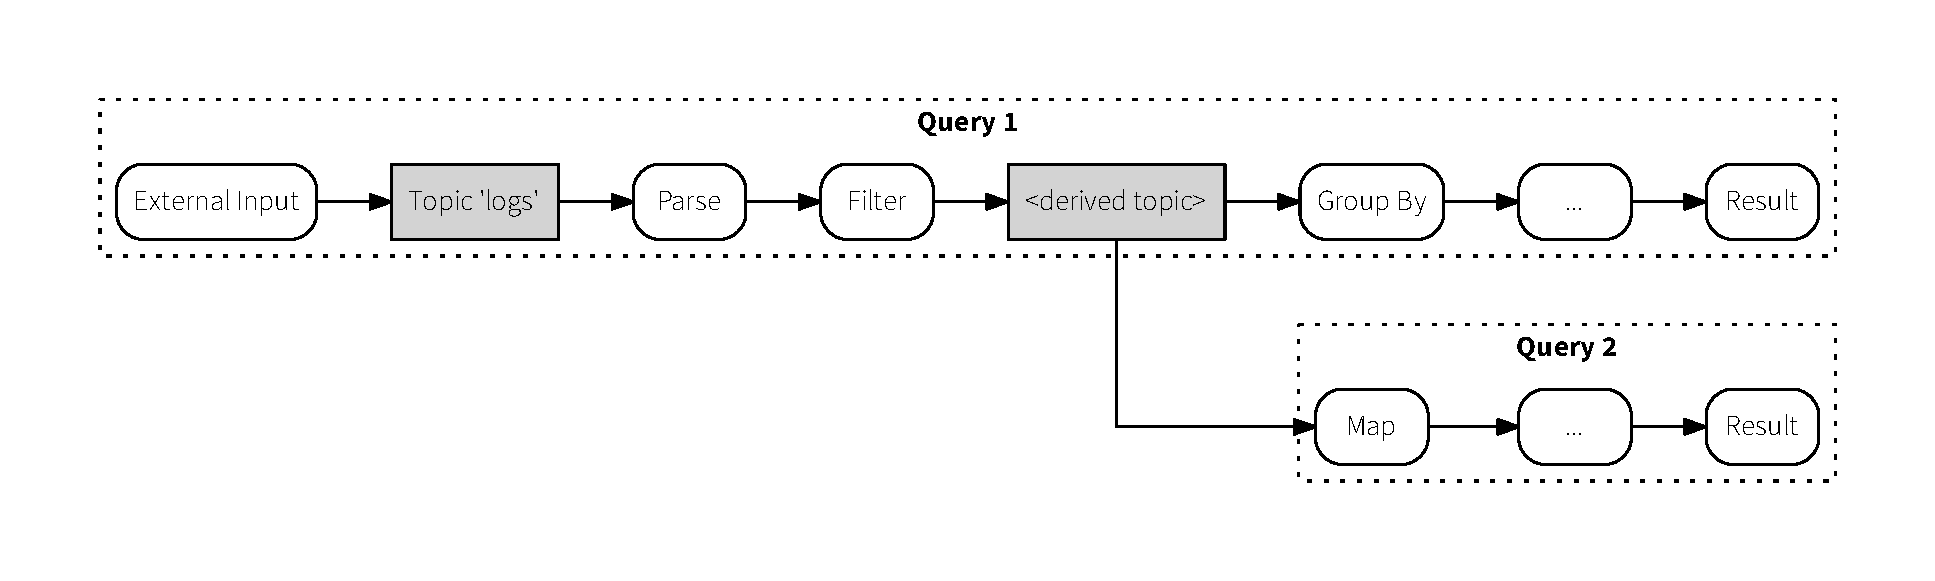
\includegraphics[scale=0.36]{figures/composition/q1q2_auto}
  \caption{Query optimization based on topic derivation. For identical
  operations on the same topic, the system would optimize the second
  query to avoid duplicated work.}
  \label{fig:queryoptimization}
\end{figure}




\subsection{Resource Management}

For the most part, resource management is still an unsolved problem in our
system: The placement of queries on executors is left to the submitting user.
While we believe that having this option is necessary: As discussed above, 
our system does not know much about the submitted queries, and thus does not
know what conditions have to be fulfilled for a good placement. In addition,
the submitting user might also always have external knowledge about the
available machines which is not expressed in the catalog.

However, in many cases automatic placement of queries is still desired. Future
work would have to explore what kind of information a query scheduler needs
from the executors to perform its task. In addition to monitoring, executors
could also control the resources allocated to a query, i.e. by using Linux
\emph{cgroups} \cite{cgroups} to ensure fair use of the available resources
by the running queries.

\subsection{Buffering and Backpressure}

If subscribers are connected, the publisher will buffer outgoing data for them
until the subscribers consume it or disconnect. This however can become an issue
if a single subscribers are slower than the publisher, as its queue grows and
memory consumption increases.

Our system allows that two queries subscribe from each other. Tightly coupled
queries thus can mitigate this problem by having the producer subscribe to
a \textquote{progress topic} published by the consumer. Future work could
explore more explicit mechanisms for notifying the publisher that it has to
slow down.

Another approach to deal with slow subscribers could be the introduction of
intermediate buffers close to the subscriber, a task typically done by the
message broker in other publish/subscribe systems. These buffers could
implement their own strategy how they want do deal with slow subscribers,
such as spilling to disk, or trying to restart slow subscribers with more
workers.

Intermediate buffers could be used to reduce network traffic, by having
multiple subscribers read their data from the local buffer instead remote
publishers.



\subsection{Persistence and Fault Tolerance}

\TODO{Timely Dataflow currently does not provide any means of fault tolerance. While
Naiad \cite{naiad} provided fault tolerance on the operator level, future work
could explore an implementation on the query level.}

\subsection{Partitioning and Filtering by Subscribers}

\TODO{In our current system, the partitioning scheme of published topics is
determined by the publishers. Kafka Streams and MillWheel both allow subscribers 
to provide partitioning functions which are used to decide how data is routed
from the publisher partitions to the subscriber instances.

This is also somewhat similar to content-based subscription.}

\clearpage
\section{Conclusions}
